%preamble - package inclusion and set up
\documentclass[12pt,twoside,a4paper,english]{report} %normal 12pt
% Select encoding of your inputs
\usepackage[utf8]{inputenc}
% Make latex understand and use the typographic
% rules of the language used in the document.
%\usepackage[danish]{babel}
\usepackage[english]{babel}

% Use the vector font Latin Modern which is going
% to be the default font in latex in the future.
%\usepackage{lmodern}
\usepackage{mathptmx}

% Choose the font encoding
\usepackage[T1]{fontenc}

% Use color in tables
\usepackage[table]{xcolor}
\usepackage{pbox}
\usepackage{tabularx}
\usepackage{array}
\usepackage{multirow}

% Load a colour package
\usepackage{xcolor}
\definecolor{aaublue}{RGB}{33,26,82}  %<--define aaublue
\definecolor{white}{RGB}{255,255,255} %<--define white

% ref stuffz			original position
%\usepackage{cleveref}

% The standard graphics inclusion package
\usepackage{graphicx}

\makeatletter
  \g@addto@macro\@floatboxreset\centering %<--centering all figures
\makeatother

\usepackage{adjustbox}

% Set up how figure and table captions are displayed

\usepackage{float}
\restylefloat{figure}
\usepackage{caption}
\usepackage{subfigure}
\usepackage[subfigure]{tocloft}
\captionsetup
{
  %justification = centering,    %<--centering caption with multiple lines
  %justification = raggedright,  %<-- right alings caption with multiple lines
  justification = justified,  %<-- justify alings (make left and right side equal) caption with multiple lines
  font          = footnotesize, %<--set font size to footnotesize
  labelfont     = bf            %<--bold label (e.g., Figure 3.2) font
}
\captionsetup[subfigure]
{
  justification = centering, %<--centering subfigure caption text
  singlelinecheck=false,
  font = footnotesize        %<--font size for subfigures
} 

% Enable row combination in tables
\usepackage{multirow}

% Make space between table lines and text
\renewcommand{\arraystretch}{1.5}

% Enable commands like \st (strike out) and \hl (high light)
\usepackage{soul}

% Make the standard latex tables look so much better
\usepackage{array,booktabs}

% Enable the use of frames around, e.g., theorems
% The framed package is used in the example environment
\usepackage{framed}
\usepackage{colortbl}
\usepackage{longtable}
\usepackage{xcolor}
\usepackage{textcomp}

%-------MATHEMATICS---------------------------------
% Defines new environments such as equation,
% align and split 
\usepackage{amsmath}
\usepackage{relsize}
% Adds new math symbols
\usepackage{amssymb}
% Use theorems in your document
% The ntheorem package is also used for the example environment
% When using thmmarks, amsmath must be an option as well. Otherwise \eqref doesn't work anymore.
\usepackage[framed,amsmath,thmmarks]{ntheorem}
\usepackage{xifthen}%<--enables ifthenelse which is used in macros

\usepackage{siunitx} 
\sisetup{decimalsymbol=period}%<--\num{} will swich commas with periods
\sisetup{detect-weight}
%---------------------------------------------------

%-------PAGE LAYOUT---------------------------------
% Change margins, papersize, etc of the document
\usepackage[
  left=25mm,% left margin on an odd page %tidligere 25mm for baade right og left
  right=25mm,% right margin on an odd page
  top=35mm,
  ]{geometry}
  
% Modify how \chapter, \section, etc. look
% The titlesec package is very configureable
\usepackage{titlesec}
\makeatletter
\def\ttl@mkchap@i#1#2#3#4#5#6#7{%
    \ttl@assign\@tempskipa#3\relax\beforetitleunit
    \vspace{\@tempskipa}%<<<<<< REMOVE THE * AFTER \vspace
    \global\@afterindenttrue
    \ifcase#5 \global\@afterindentfalse\fi
    \ttl@assign\@tempskipb#4\relax\aftertitleunit
    \ttl@topmode{\@tempskipb}{%
        \ttl@select{#6}{#1}{#2}{#7}}%
    \ttl@finmarks  % Outside the box!
    \@ifundefined{ttlp@#6}{}{\ttlp@write{#6}}}
\makeatother

\titlespacing{\chapter}{0pt}{0pt}{10pt}
\titlespacing{\section}{0pt}{0pt}{-5pt}
\titlespacing{\subsection}{0pt}{8pt}{-5pt}
\titlespacing{\subsubsection}{0pt}{6pt}{-10pt}

\titleformat*{\section}{\normalfont\Large\bfseries\color{aaublue}}
\titleformat*{\subsection}{\normalfont\large\bfseries\color{aaublue}}
\titleformat*{\subsubsection}{\normalfont\normalsize\bfseries\color{aaublue}}

\usepackage{titlesec, blindtext, color}
%\color{gray75}{gray}{0.75}
\newcommand{\hsp}{\hspace{20pt}}
\titleformat{\chapter}[hang]{\Huge\bfseries}{\thechapter\hsp\textcolor{aaublue}{|}\hsp}{0pt}{\Huge\bfseries}

% Change the headers and footers
\usepackage{fancyhdr}
\setlength{\headheight}{15pt}
\pagestyle{fancy}
\fancyhf{} %delete everything
\renewcommand{\headrulewidth}{0pt} %remove the horizontal line in the header
\fancyhead[RO,LE]{\color{aaublue}\small\nouppercase\leftmark} %even page - chapter title
\fancyhead[LO]{}
\fancyhead[RE]{} 
\fancyhead[CE]{}
\fancyhead[CO]{}
\fancyfoot[RE,LO]{\thepage}
\fancyfoot[LE,RO]{} %page number on all pages
\fancyfoot[CE,CO]{}

% change first page of all chapters header and footer to fancy style
\makeatletter
\let\ps@plain\ps@fancy
\makeatother

% Do not stretch the content of a page. Instead,
% insert white space at the bottom of the page
\raggedbottom

% Enable arithmetics with length. Useful when typesetting the layout.
\usepackage{calc}
%---------------------------------------------------

\usepackage{appendix}

%-------BIBLIOGRAPHY--------------------------------
%setting references (using numbers) and supporting i.a. Chicargo-style:
\usepackage{etex}
\usepackage{etoolbox}
\usepackage{keyval}
\usepackage{ifthen}
\usepackage{url}
\usepackage{csquotes}
\usepackage[backend=bibtex, isbn=false, url=false, eprint=false, doi=false, style=numeric, sorting=none]{biblatex}
\addbibresource{setup/Canada-Project.bib}
%---------------------------------------------------

%-------MISC----------------------------------------
%%% Enables the use FiXme refferences. Syntax: \fxnote{...} %%%
\usepackage[footnote, draft, english, silent, nomargin]{fixme}		%>>>> draft OR final <<<< 
%With "final" instead of "draft" an error will ocure for every FiXme under compilation.

%%% allows use of lorem ipsum (generate i.e. pagagraph 1 to 5 with \lipsum[1-5]) %%%
\usepackage{lipsum}

%%% Enables figures with text wrapped tightly around it %%%
\usepackage{wrapfig}

%%% Section debth included in table of contents (1 = down to sections) %%%
\setcounter{tocdepth}{1}

%%% Section debth for numbers (1 = down to sections) %%%
\setcounter{secnumdepth}{2}

\usepackage{tocloft}
\setlength{\cftbeforetoctitleskip}{0 cm}
\renewcommand{\cftpartpresnum}{Del~}
\let\cftoldpartfont\cftpartfont
\renewcommand{\cftpartfont}{\cftoldpartfont\cftpartpresnum}
%---------------------------------------------------

%-------DANSK SPROG---------------------------------

%\addto\captionsdanish{%
%	\renewcommand{\figurename}{figur}%
%	\let\figureautorefname\figurename%
%	\renewcommand{\tablename}{tabel}%
%	\let\tableautorefname\tablename%
%%	\renewcommand{\equationname}{ligning}%
%%	\let\equationautorefname\equationname%
%	\renewcommand{\chaptername}{Kapitel}%
%	\let\chapterautorefname\chaptername%
%	\renewcommand{\partname}{Del}%
%	\let\partautorefname\partname%
%	\renewcommand{\sectionname}{afsnit}%
%	\let\sectionautorefname\sectionname%
%%	\renewcommand{\thesubsection}{underafsnit}%
%%	\let\subsectionautorefname\thesubsection%
%	\renewcommand{\pagename}{side}%
%	\let\pageautorefname\pagename%
%}

%-------HYPERLINKS----------------------------------
% Enable hyperlinks and insert info into the pdf
% file. Hypperref should be loaded as one of the 
% last packages
\usepackage{nameref}
\usepackage{hyperref}
\usepackage{bookmark}
\hypersetup{%
	%pdfpagelabels=true,%
	plainpages=false,%
	pdfauthor={Author(s)},%
	pdftitle={Title},%
	pdfsubject={Subject},%
	bookmarksnumbered=true,%
	colorlinks,%
	citecolor=aaublue,%
	filecolor=aaublue,%
	linkcolor=aaublue,% you should probably change this to black before printing
	urlcolor=aaublue,%
	pdfstartview=FitH%
}

% ref stuffz		new position
\usepackage{cleveref}

\crefname{appsec}{bilag}{bilag}
%---------------------------------------------------



% remove all indentations
\setlength\parindent{0pt}
\parskip 5mm
\usepackage{verbatim}

\definecolor{Gra}{RGB}{230,230,230}

%creates a nice-looking C#-text
\newcommand{\CC}{C\nolinebreak\hspace{-.05em}\raisebox{.3ex}{\scriptsize\text \#} }

%enables multi column lists
\usepackage{multicol}

%enables code-examples
\usepackage{listings}

\definecolor{coolblue}{RGB}{32,95,128}
\definecolor{mygreen}{rgb}{0,0.6,0}
\definecolor{mygray}{rgb}{0.5,0.5,0.5}
\definecolor{mymauve}{rgb}{0.58,0,0.82}
\usepackage{textcomp}
\definecolor{listinggray}{gray}{0.9}
\definecolor{lbcolor}{rgb}{0.9,0.9,0.9}

%for c code
\lstdefinestyle{cstyle}{
  backgroundcolor=\color{lbcolor},
	tabsize=4,
	rulecolor=,
	language=C,
  basicstyle=\scriptsize,
  upquote=true,
  aboveskip={1.5\baselineskip},
  columns=fixed,
  showstringspaces=false,
  extendedchars=true,
  breaklines=true,
  prebreak = \raisebox{0ex}[0ex][0ex]{\ensuremath{\hookleftarrow}},
  frame=single,
  showtabs=false,
  numbers=left,
  captionpos=b,
  numbersep=5pt,
  numberstyle=\tiny\color{mygray},
  showspaces=false,
  showstringspaces=false,
  identifierstyle=\ttfamily,
  keywordstyle=\color[rgb]{0,0,1},
  commentstyle=\color[rgb]{0.133,0.545,0.133},
  stringstyle=\color[rgb]{0.627,0.126,0.941},
}
%for python code
\lstdefinestyle{pythonstyle}{
    backgroundcolor=\color{lbcolor},
    tabsize=4,
    rulecolor=,
    language=python,
    basicstyle=\scriptsize,
    upquote=true,
    aboveskip={1.5\baselineskip},
    columns=fixed,
    showstringspaces=false,
    extendedchars=true,
    breaklines=true,
    prebreak = \raisebox{0ex}[0ex][0ex]{\ensuremath{\hookleftarrow}},
    frame=single,
    showtabs=false,
    numbers=left,
    captionpos=b,
    numbersep=5pt,
    numberstyle=\tiny\color{mygray},
    showspaces=false,
    showstringspaces=false,
    identifierstyle=\ttfamily,
    keywordstyle=\color[rgb]{0,0,1},
    commentstyle=\color[rgb]{0.133,0.545,0.133},
    stringstyle=\color[rgb]{0.627,0.126,0.941},
}
%for matlab code
\lstdefinestyle{matlabstyle}{
    backgroundcolor=\color{lbcolor},
    tabsize=4,
    rulecolor=,
    language=Matlab,
    basicstyle=\scriptsize,
    upquote=true,
    aboveskip={1.5\baselineskip},
    columns=fixed,
    showstringspaces=false,
    extendedchars=true,
    breaklines=true,
    prebreak = \raisebox{0ex}[0ex][0ex]{\ensuremath{\hookleftarrow}},
    frame=single,
    showtabs=false,
    numbers=left,
    captionpos=b,
    numbersep=5pt,
    numberstyle=\tiny\color{mygray},
    showspaces=false,
    showstringspaces=false,
    identifierstyle=\ttfamily,
    keywordstyle=\color[rgb]{0,0,1},
    commentstyle=\color[rgb]{0.133,0.545,0.133},
    stringstyle=\color[rgb]{0.627,0.126,0.941},   
}

%for java code
\lstdefinestyle{javastyle}{
	backgroundcolor=\color{lbcolor},
	tabsize=4,
	rulecolor=,
	language=Java,
	basicstyle=\scriptsize,
	upquote=true,
	aboveskip={1.5\baselineskip},
	columns=fixed,
	showstringspaces=false,
	extendedchars=true,
	breaklines=true,
	prebreak = \raisebox{0ex}[0ex][0ex]{\ensuremath{\hookleftarrow}},
	frame=single,
	showtabs=false,
	numbers=left,
	captionpos=b,
	numbersep=5pt,
	numberstyle=\tiny\color{mygray},
	showspaces=false,
	showstringspaces=false,
	identifierstyle=\ttfamily,
	keywordstyle=\color[rgb]{0,0,1},
	commentstyle=\color[rgb]{0.133,0.545,0.133},
	stringstyle=\color[rgb]{0.627,0.126,0.941},
}

%for inline c, syntax: \cline{ codeHere(); }
\lstdefinestyle{cinline}{
    style=cstyle,
    basicstyle=\small,
}
\newcommand\inlinec[1]{ \lstinline[style=cinline]{#1} }

%for inline python, syntax: \pythonline{ codeHere(); }
\lstdefinestyle{pythoninline}{
    style=pythonstyle,
    basicstyle=\small,
}
\newcommand\inlinepython[1]{ \lstinline[style=pythoninline]{#1} }

%for inline matlab, syntax: \matlabline{ codeHere(); }
\lstdefinestyle{matlabinline}{
    style=matlabstyle,
    basicstyle=\small,
}
\newcommand\inlinematlab[1]{ \lstinline[style=matlabinline]{#1} }

\usepackage{enumitem}
%\usepackage[citestyle=authoryear,natbib=true]{biblatex}

% Figures - TIKZ
\usepackage{tikz}
\usepackage[americanresistors,americaninductors,americancurrents, americanvoltages]{circuitikz}

% Wall of text logo
\newcommand{\walloftextalert}[0]{\includegraphics[width=\textwidth]{walloftext.png}}

\usepackage{pdfpages}
\usepackage{lastpage}
\usepackage{epstopdf}

\setlength{\headheight}{21pt}

\hfuzz=\maxdimen
\tolerance = 10000
\hbadness  = 10000

\usepackage{siunitx}
\graphicspath{{./figures/}}

%macros - please read this file
%Macro for 'where'-enviroment was improved by Andrea and Niels :-)

%-----------UNITS-------------------------------------------
\newcommand{\unit}[1]{&& \left[\si{#1}\right]}
%
%\newcommand{\unit}[1]{[\si{#1}]}            %<<| Use these if you want equations to be
%\newcommand{\eq}[2]{&&\si{#1} &= \si{#2}&&} %<<| centered.. .. will appear scrambled
%                                            %  | from one equation to the next though..
%                                            %  | and does not work with long equations.. :/
%
%-----------------------------------------------------------

%-----------WHERE ENVIRONMENT-------------------------------
\newenvironment{where}{\leavevmode{\parindent=1em\indent} Where:\\}{}
\newcommand{\va}[3]
{
  \begin{tabular}{p{20pt} p{40pt} p{290pt} l}
    & { $#1$ } & { #2 } & \ifthenelse{\isempty{ #3 }}  {}  {[{\si{#3}}]} \\
  \end{tabular}\\
}
%-----------------------------------------------------------

%-----------TikZ SETTINGS-----------------------------------
\tikzset{
  block/.style    = {draw, thick, rectangle,
                     minimum height = 2.1em,
                     minimum width = 1.7em},
  sum/.style      = {draw, circle, inner sep=3pt} %<--Adder
}
%-----------------------------------------------------------


%-----------Fanzy reference SETTINGS------------------------
%Figure references:
\newcommand{\figref}[1]{figure \ref{#1}}

%Figure references after full stop/period:
\newcommand{\Figref}[1]{Figure \ref{#1}}

%Table references:
\newcommand{\tabref}[1]{table \ref{#1}}

%Table references after full stop/period:
\newcommand{\Tabref}[1]{Table \ref{#1}}

%Section references:
\newcommand{\secref}[1]{section \ref{#1}} % on page \pageref{#1}}

%Section references:
\newcommand{\Secref}[1]{Section \ref{#1}} % on page \pageref{#1}}

%Subsection references:
\renewcommand{\subref}[1]{section \ref{#1}} % on page \pageref{#1}}

%Subsection references:
\renewcommand{\Subref}[1]{Section \ref{#1}} % on page \pageref{#1}}

%Appendix references:
\newcommand{\appref}[1]{appendix \ref{#1}} % on page \pageref{#1}}

%Appendix references:
\newcommand{\Appref}[1]{Appendix \ref{#1}} % on page \pageref{#1}}

%chapter references: 
\newcommand{\chapref}[1]{chapter \ref{#1}} % on page \pageref{#1}}

%chapter references: 
\newcommand{\Chapref}[1]{Chapter \ref{#1}} % on page \pageref{#1}}

%Units:
%\newcommand{\unit}[1]{&& \left[\si{#1}\right]}

%Text:
\newcommand{\tx}[1]{\text{#1}}

%Equation references:
%1 equation:
\renewcommand{\eqref}[1]{equation (\ref{#1})}

%-----------------------------------------------------------





\begin{document}       % TIP: If you are using TeXstudio you can open
%\tableofcontents      %      the file by Ctrl+LeftClick on setup/macros.tex
%\pagebreak             %      If the file doesn't exist, you will be asked
					   %      weather or not you want to create it.
%\begin{center}
%	\vspace{5cm}
%	\Huge{Worksheets}
%\end{center}
%\clearpage

%||||||||||||||||||||||||||||||||||||||||||||||||||||||||||||||||
%|||||||                 Example Inputs                  ||||||||
%||||||||||||||||||||||||||||||||||||||||||||||||||||||||||||||||
%|||||||                                                 ||||||||
%			 \chapter{Figure Sample}

\begin{figure}[H]                                         %   File-type can be specified
  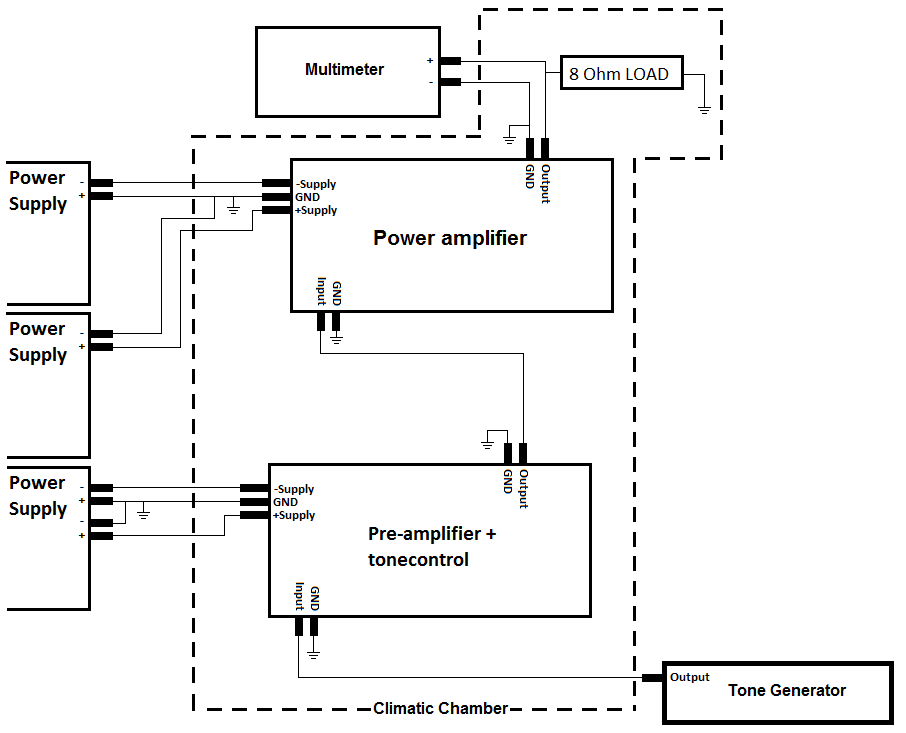
\includegraphics[width=.4\textwidth]{figures/filename}  %<--but is not needed.
  \caption{This image is clearly too small, remember to scale appropriately \fxnote{Remember source}}
  \label{fig:FigureLABEL}  %<--give the figure a label, so you can reference!
\end{figure}               %   For the label to work it must be under the caption.

% Fxnotes will not compile properly inside the figure, only in the caption.
% When \fxnote{} is used in caption, it does not show in a footnote as it normally 
% would, it does however appear in list of corrections.

\autoref{fig:FigureLABEL} $\leftarrow$ use autoref, unless you are referring to multiple pictures, then do like this: \autoref{fig:HbridgeClokwise4Q} and \ref{fig:HbridgeCounterClokwise4Q}.

%Do NOT use \vspace{length}, \hspace{length} or \noindent etc. unless exceedingly necessary - LaTeX is a markup language, let it do its job.
\vspace{.5cm}
\noindent
%
%--------- BIBLIOGRAPHY REF EKSAMPLE -----------------------------------
This reference only represents this line since it is before the punctuation mark\cite{YDing}. This next reference however represents the entire section. That is, all of the preceding sentences in the entire section. This is due to the fact that it is now after the punctuation mark in the end of the section (this is not used in the middle of a section!).\cite{YDing}

%>>PLEASE ALSO READ THE NOTE IN bibliography/bibliography.bib<<

Here is a way to make two images appear on the side of each other. Also, if you modified an image, this is how you properly refer to its original source:

\begin{figure}[H]
    \subcaptionbox  %<--use captionbox instead if no global caption is needed
    {               %                                \%-%-%-%-%-%-%\
      Clockwise 4Q operation.\newline                              %\
      \emph{Edited from image by Biezl.\cite{Biezl}}                %\
      \label{fig:HbridgeClokwise4Q}                                  %\
    }                                                                 %\
    {                                                                  %\
      \includegraphics[width=.46\textwidth]{HbridgeClockwise4Q}         %\
    }                                                                    %\
    \hspace{5pt}                                                          %\
    \subcaptionbox  %<-----------------------------------------------------%\
    {                                                                       %\
      Counterclockwise 4Q operation.\newline                                 %\
      \emph{Edited from image by Biezl.\cite{Biezl}}                          %\
      \label{fig:HbridgeCounterClokwise4Q}                                     %\
    }                                                                           %\
    {                                                                            %\
      \includegraphics[width=.46\textwidth]{HbridgeCounterClockwise4Q}            %|
    }                                                                             %|
    \caption{The 4 quadrant H-bridge configuration shown in both directions.}%<-%-/
    \label{fig:Hbridges}
\end{figure}

As seen \autoref{fig:HbridgeCounterClokwise4Q} can be referred to on its own, or you can use \autoref{fig:Hbridges} to refer to both \autoref{fig:HbridgeClokwise4Q} and \autoref{fig:HbridgeCounterClokwise4Q}.

If the figures are not directly related you might not want to use \textbf{(a)} and \textbf{(b)}, but instead give each figure their own label, here is an example:

\begin{figure}[H]
    \captionbox
    {
      Clockwise 4Q operation.\newline
      \emph{Edited from image by Biezl.\cite{Biezl}}
      \label{fig:HbridgeClokwise4Q2}
    }
    {
      \includegraphics[width=.46\textwidth]{HbridgeClockwise4Q}
    }
    \hspace{5pt}
    \captionbox
    {
      Counterclockwise 4Q operation.\newline
      \emph{Edited from image by Biezl.\cite{Biezl}}
      \label{fig:HbridgeCounterClokwise4Q2}
    }
    {
      \includegraphics[width=.46\textwidth]{HbridgeCounterClockwise4Q}
    }
\end{figure}

In this case \autoref{fig:HbridgeClokwise4Q2} can be referred to without involving \autoref{fig:HbridgeCounterClokwise4Q2}.

\pagebreak			 %|||||||
%			 \section{Table Sample} %to view this sample properly in the code, the screen must be
                       %wide enough, or you have to disable word-wrap in your editor.
\begin{table}[H]
\begin{tabular}{|l|p{5cm}|l|l|l|}
  \hline %-----------------------------------------------------------------------------------
  \textbf{No.} &\textbf{Description} &\textbf{Min} &\textbf{Max} &\textbf{Requirements}    \\
  \hline %-----------------------------------------------------------------------------------
  1            & Some Text           & Some Text   & Some Text   & Some Text               \\
               &                     &             &             & Some More Text          \\
               &                     &             &             & Text Text               \\
               &                     &             &             & Text Text Text          \\
  \hline %-----------------------------------------------------------------------------------
  2            & Some Text           & Some Text   & Some Text   & Some Text               \\
  \hline %-----------------------------------------------------------------------------------
  3            & By specifying the
                 width of a column
                 (|p\{5cm\}|) the
                 cells in that column
                 will not exceed the
                 specified width but         %Extra whitespace is used only for clarity
                 instead expand              %and will not affect the compiled output.
                 downward.
                                     & Some Text           & Some Text   & Some Text       \\
  \hline %-----------------------------------------------------------------------------------
  4            & Some Text           & Some Text   & Some Text   & Some Text               \\
  \hline %-----------------------------------------------------------------------------------
  \multicolumn{2}{|l|}{Some Text}    & \multicolumn{3}{l|}{Some Text}                      \\
  \hline %-----------------------------------------------------------------------------------
  \multicolumn{2}{|l|}{Text Text}    & \multicolumn{3}{l|}{Text = Text}                    \\
  \multicolumn{2}{|l|}{}             & \multicolumn{3}{l|}{Text = Text}                    \\
  \multicolumn{2}{|l|}{}             & \multicolumn{3}{l|}{Text = Text}                    \\
  \multicolumn{2}{|l|}{}             & \multicolumn{3}{l|}{Text = Text}                    \\
  \multicolumn{2}{|l|}{}             & \multicolumn{3}{l|}{Text = Text}                    \\
  \hline %-----------------------------------------------------------------------------------
  \multicolumn{2}{|l|}{Some Text}    & \multicolumn{3}{l|}{Teeeexxtt}                      \\
  \multicolumn{2}{|l|}{}             & \multicolumn{3}{l|}{\LaTeX}                         \\
  \hline %-----------------------------------------------------------------------------------
\end{tabular}
\caption{This Is a Table\label{table:TableLABEL}}
\end{table}

\autoref{table:TableLABEL} $\leftarrow$ use autoref, unless you are referring to multiple tables, then do like this: \autoref{table:TableLABEL} and \ref{table:TableLABEL}.

\pagebreak 		     %|||||||
%			 \section{Equation Sample} %<--In American English all Important Words in
                          %   Headlines are with Big Letters

% \unit is a macro. It uses SI units and aligns all the units neatly :)

\textbf{A normal equation:}
\begin{flalign}
  J_m \cdot \dot{\omega}_m(t) &= \tau_m(t) - B_m \cdot \omega_m(t) - r_m \cdot f_c(t)& \unit{N \cdot m}
  \label{eq:MotorGearNewtonSecLaw}
\end{flalign}
%
\begin{where}
  \va{ J_m               }{is the motor's inertia}                     {kg \cdot m^2}
  \va{ \omega_m(t)       }{is the angular velocity of the motor}       {rad \cdot s^{-1}}
  \va{ \dot{\omega}_m(t) }{is the angular acceleration of the motor}   {rad \cdot s^{-2}}
  \va{ \tau_m(t)         }{is the torque delivered by the motor}       {N \cdot m}
  \va{ B_m               }{is the motor's friction coefficient}        {N \cdot m \cdot s \cdot rad^{-1}}
  \va{ r_m               }{is the radius of the gear, $G_m$}           {m}
  \va{ f_c(t)            }{is the contact force between the two gears} {N}
\end{where}

\textbf{If you need to write something with numbers:} %<--Do not use \textbf{} as headlines, it is bad practice
                                                      %   use instead \chapter{}, \section{}, \subcaption{}, \subsubsection{}
                                                      %   in that order - never a \subsubsection{} directly under a \section{}
\begin{flalign}
  B      &= \num{2,2}\cdot 10^{-6}  \ \si{N\cdot m \cdot rad^{-1} \cdot s}& \label{eq:eq2} \\ %<-- if you want two equations to
  \tau_c &= \num{0.0016}            \ \si{N\cdot m}                       & \label{eq:eq3}    %    allign in one envirenment,
\end{flalign}                                                                              %    remember \\
%using \num{} ensures the same use of decimal point throughout the repport
%should you want to change it, the option is set in the preamble, just change 'period' to 'comma':
%\sisetup{decimalsymbol=period}

\autoref{eq:MotorGearNewtonSecLaw} $\leftarrow$ use autoref, unless you are referring to multiple equations, then do like this: \autoref{eq:eq2} and \ref{eq:eq3}.

\pagebreak		 %|||||||
%			 \section{TikZ Sample}

\textbf{TikZ is only for very patient people, I can recommend Inkscape with textext plugin: \url{https://pav.iki.fi/software/textext/}, difficult to install easy to use, and, if used carefully, nice results.}

%heavily commented example
\input{chapters/tikz/TikZblockDiagramSample.tex}

%way to keep the drawing code in a seperate file
\begin{figure}[H]
	\input{chapters/tikz/smallBlockDiagram.tikz}
	\centering
	\caption{Block diagram}
\end{figure}

%TikZ can also be used for circuits
\input{chapters/tikz/TikZcircuitSample.tex}


\pagebreak            %|||||||
%			 \section{Code Sample}

\begin{lstlisting}[ style=cstyle,
                    caption={C Code}, 
                    label=lst:cExample ]
#include "functions.h"

// Constant matrices
const float L[3] = { -11.0, -12.0, -13.0 };
const float B1[4] = { 0.0, -0.2396, 0.0, 0.2396 };
const float B2[4] = { 0.2396, 0.0, -0.2396, 0.0 };
const float B3[4] = { 0.0377, -0.0377, 0.0377, -0.0377 };
\end{lstlisting}

In \autoref{lst:cExample} is some C-code, and here is some in-line C-code: \inlinec{xTaskCreate();}.

\begin{lstlisting}[ style=pythonstyle,
                    caption={Python Code}, 
                    label=lst:pythonExample ]
# This parses the packets to identify messages and decodes them for the logs
class packetParser():
    def __init__(self,accelfile,gpsfile,measstate,fulllog,plog):
        self.GPS = {0: 'Latitude',
                    1: 'Longtitude',
                    2: 'Velocity'}
        self.IMU = {0: 'AccelerationX',
                    1: 'AccelerationY',
                    2: 'AccelerationZ',
                    3: 'GyroscopeX',
                    4: 'GyroscopeY',
                    5: 'GyroscopeZ',
                    6: 'MagnetometerX',
                    7: 'MagnetometerY',
                    8: 'MagnetometerZ',
                    9: 'Temperature'}
        self.MsgID = {0: self.GPS, 1: self.IMU}
        self.DevID = {0: 'GPS', 1: 'IMU'}
        self.accelburst = [0,0,0,0,0,0,0]
        self.accellog = accelfile
        self.fulllog = fulllog
\end{lstlisting}

In \autoref{lst:pythonExample} is some Python-code, and here is some in-line Python-code:\\ \inlinepython{self.plog.write(str(msgnr))}

\begin{lstlisting}[ style=matlabstyle,
                    caption={Matlab Code}, 
                    label=lst:matlabExample ]
  close all
  clear
  clc
  
  % Parameters
  mx=200;     % [kg] mass + added mass in xb direction
  my=250;     % [kg] mass + added mass in yb direction
  Iz=700;     % [kgm2]
  
  dx=70;      % [kg/s] 
  dy=100;     % [kg/s]
  dyaw=50;    % [kgm2/s]
\end{lstlisting}

In \autoref{lst:cExample}, \ref{lst:pythonExample} and \ref{lst:matlabExample} is some code, and here is some in-line matlab: \inlinematlab{randn(50)}            %|||||||
%|||||||                                                 ||||||||
%||||||||||||||||||||||||||||||||||||||||||||||||||||||||||||||||
%||||||||||||||||||||||||||||||||||||||||||||||||||||||||||||||||


%%% Prereport %%%
		\setlength\cftaftertoctitleskip{2pt}
		\setlength\cftafterloftitleskip{6pt}
		\setlength\cftafterlottitleskip{6pt}
%\selectlanguage{danish}
%\title{Testing the performance of linear regressors using inertial information combined with sEMG to minimize the limb position effect in proportional and simultaneous control of lower arm prosthetics.}

%%% Frontmatter Settings %%%
		\pagestyle{empty} %disable headers and footers
		\pagenumbering{roman} %use roman page numbering in the frontmatter I II...
%		\fancyfoot[RE,LO]{17gr7404} %page number on all pages
%		\fancyfoot[LE,RO]{\thepage}
%		\fancyhead[LE,LO,RE,RO]{}

%%% Introductory Formalities %%%
%\includepdf[pages={1}]{formalities/frontpage.pdf}
			\clearpage
\thispagestyle{empty}

\begin{figure}[H]
	\raggedleft{
	
\includegraphics[width=0.3\textwidth]{setup/aaulogo-en.png} }
	\hspace{4.5cm}
	\raggedright{
	
\includegraphics[width=0.35\textwidth]{setup/RNL.png} }
\end{figure} 

\vspace{3 cm}

\begin{center}
	\begin{Huge}
	%	\textbf{- Status Seminar -}\\
	%	\vspace{2cm}
		\textbf{Developing a wearable system to assess balance during advanced dynamic movements}\\ 
	\end{Huge}
%\vspace{5mm}
%\begin{Large}
%	\textbf{- A pilot study -}\\
%\end{Large}
		\vspace{20 mm}
		\begin{Huge}
		3rd semester Masters, Biomedical Engineering \& Informatics - Autumn $2018$\\
		\vspace{3 mm}
	\end{Huge}
	{\Large Project group: $18$gr$9406$} \\
	\vspace{1cm}
	\large{Simon Bruun and Oliver Thomsen Damsgaard}
\end{center}
\vspace*{\fill}

\begin{center}
	\line(1,0){400}
\end{center}

%\newpage
%
%\large{\textbf{Project period:}\\
%P7, Autumn 2017\\
%01/08/2017 - 20/12/2017\\
%
%\textbf{Project group:}\\
%17gr7404\\} %\fxnote{Input group number}
%
%
%\begin{center}
%	\Large{\textbf{Collaborators:}\\
%		\vspace{1.5cm}
%	\rule{10cm}{1pt}\\
%	Irene Uriarte \\
%	
%	\rule{10cm}{1pt}\\
%	Martin Alexander Garenfeld \\
%	
%	\rule{10cm}{1pt}\\
%	Oliver Thomsen Damsgaard \\
%	
%	\rule{10cm}{1pt}\\
%	Simon Bruun \\}
%\end{center}
%
%
%
%\large{\textbf{Supervisors:}\\
%Strahinja Dosen \\
%Jakob Lund Dideriksen \\
%Lotte N.S. Andreasen Struijk} \\
%\\
\newpage
			% <--- the frontpage
%			\pagestyle{fancy}
%%{\small
\strut\vfill % push the content to the bottom of the page
\noindent Copyright \copyright{} Aalborg University 2015\par
\vspace{0.2cm}

\noindent This report is compiled in \LaTeX, originally developed by Leslie Lamport, based on Donald Knuth's \TeX. The main text is written in \emph{Latin Modern} pt 12, designed by Bogusław Jackowski and Janusz M. Nowacki. 
%The document is compiled via the website \url{www.overleaf.com}, an online collaborative based \LaTeX-editor with instant preview, which enables multiple persons to edit the document simultaneously.
Flowcharts and diagrams are made using Microsoft Visio. 
\clearpage
%			%\begin{document} 
\thispagestyle{empty}
\begin{titlepage}
%\begin{nopagebreak}
{\samepage 

\begin{tabular}{r}
\parbox{\textwidth}{  \raisebox{-15mm}{
\includegraphics[height=3cm]{setup/aaulogo-en.png}}
\hfill \hspace{2cm} \parbox{8cm}{\begin{tabular}{l} %4.90
{\small \textbf{\textcolor{aaublue}{{9\textsuperscript{th} Semester, Masters Project}}}}\\
{\small \textbf{\textcolor{aaublue}{School of Medicine and Health}}}\\
%{\small \textbf{\textcolor{aaublue}{Communication Technologies}}}\\ 
{\small \textbf{\textcolor{aaublue}{Biomedical Engineering and Informatics}}}\\
{\small \textcolor{aaublue}{Fredrik Bajers Vej 7A}} \\
{\small \textcolor{aaublue}{9220 Aalborg}} \\
%{\small \textcolor{aaublue}{\emph{http://www.sict.aau.dk/electronics-and-it}}}
\end{tabular}}}
\end{tabular}}

\begin{tabular}{r}
%\parbox{7cm}{

%\textbf{The effect of limb position on myoelectric prosthetic control using linear regression}
%\\
%\textbf{Theme: Biomedical signals and information}

%\small{
%\\
%}


\parbox{5cm}{


\textbf{Project period:}\\
P7, Autumn 2017\\
01/08/2017 - 20/12/2017\\
   
\textbf{Project group:}\\
17gr7404\\ %\fxnote{Input group number}
  
\textbf{Collaborators:}\\
%\rule{5cm}{1pt}\\
%Irene Uriarte \\
%\rule{5cm}{1pt}\\
%Martin Alexander Garenfeld \\
\rule{5cm}{1pt}\\
Simon Bruun \\
\rule{5cm}{1pt}\\
Oliver Thomsen Damsgaard \\


\textbf{Supervisors:}\\
Strahinja Dosen \\
Jakob Lund Dideriksen \\
Lotte N.S. Andreasen Struijk \\
}\\


\textbf{Pages:} 0\\
\textbf{Appendixes:} b \\
%\textbf{Ekstra:} For projektkode: Se forord\\ %eks. en CD eller USB
\textbf{Completed:} 19/12/2017\\

%\end{tabular}


%\vfill &
%\parbox{1cm}{
  %\vspace{.15cm}
  %\hfill
  
  \begin{tabular}{l}
  %{\textbf{Abstract}}\bigskip \\
  \fbox{
    \parbox{6cm}{\bigskip
     {\vfill{\small \lipsum[15]
%write real thing
     \bigskip}}
     }}
   \end{tabular} }

\end{tabular} %\vspace{1cm}



\centering
\textit{Publication of this report's contents, including source references, may only happen in agreement with the authors.}\\
%\textit{Offentliggørelse af rapportens indhold, med kildeangivelse, må kun ske efter aftale med forfatterne.}\\


%\end{nopagebreak}
\end{titlepage}
%\end{document} 			 % <--- the titlesheet - contains the synopsis!!
%%%% Preface %%%
%			\cleardoublepage
%			\lipsum[15]
%write real thing			 % <--- this is the abstract!!
%%\clearpage
%			\chapter*{Preface}

\lipsum[9]

\pagebreak				% <--- the preface
%

\clearpage
			\pdfbookmark[0]{Table of Contents}{label: tableOfCentents}
			\tableofcontents
			\cleardoublepage


%%% Mainmatter Settings %%%
\pagenumbering{arabic} %use arabic page numbering in the mainmatter
\fancyhf{}
\fancyfoot[C]{\thepage} %\text{ of} \pageref{LastPage}			% ADD LABLE{LASTPAGE} TO LAST PAGE !!
\fancyfoot[RE,LO]{18gr9406}																								   %
\fancyhead[RE,LO]{}																												%% } consider fancyfoots
\fancyhead[RE,LO]{\color{aaublue}\small\nouppercase\leftmark} %even page - chapter title %
\pagestyle{fancy}


%---------------------------INPUTS-------------------------------

%\input{contents/statusText.tex}
%\chapter{Introduction} \label{chap:Introduction}



\chapter{Problem Analysis} \label{chap:PA}

%stroke

\section{Cardiovascular Diseases}

%Short introduction to cvd, stroke and the two subtypes
Cardiovascular diseases (CVD) are the number one cause of death on a world wide scale. In 2015 CVDs was estimated to account for more than 31\% of all deaths globally. \cite{whocvd2017} CVD are a collected term for a number of conditions revolving around diseases to the heart and system of blood vessels. According to the World Health Organisation (WHO) the top two causes of global deaths are the CVDs coronary artery disease and stroke. Of the two, stroke accounted for 10\% of deaths in 2016. \cite{whoMortalityStats2018}

%something on why we focus on stroke rather than coronary artery disease...?

\subsection{Stroke}
%stroke in numbers and causes /cites: (Hering2016chap7 and 8), Mackay2002, Sharma2017
A stroke is caused by either a blockage or rupture of blood vessels in the brain. As such stroke is divided into two subtypes; ischaemic stroke and haemorrhagic stroke. During a ischaemic stroke a blood vessel in the brain is blocked by blood cloths caught in narrow blood vessels. The narrowing of blood vessels are commonly caused by other conditions such as high cholesterol, high blood pressure, unhealthy lifestyle and ageing. If a blood vessel is blocked a part of the brain will be shot off from its blood supply. If not treated within minutes this can cause damage to brain cells in the cut-off area. \cite{Mackay2002, Hering2016chap7, InternetStroke2018} 
During an haemorrhagic stroke a blood vessel will rupture and blood will leak inside the brain. Depending on where in the brain the leak occurs the haemorrhagic stroke is either a intracerebral haemorrhage or and subarachnoid haemorrhage, intracerebral being inside the brain and subarachnoid occurring in the space between the brain and the cranium. In both types a rupture and leakage of blood can cause a sudden increase in pressure potentially causing damage to brain cells and can lead to sudden unconsciousness and death. The most common causes are high blood pressure, unhealthy lifestyle, diabetes and ageing. \cite{Mackay2002, Hering2016chap8, InternetStroke2018}

\subsection{Stroke Complications}
%post stroke consequences \cite{Sharma2017}
%outcomes/consequences, damages to balance/coordination of movements /cites: Bhalla2016, Sharma2017
Complications following a stroke are common. In surviving patients 30-96\% have been reported to experience post-stroke complications of both physical and psychological nature. Complications involve recurrent stroke and epileptic seizures, cardiac arrhythmias and failure, infections, problems in gastrointestinal and genitourinary systems, complication of immobility, dementia, pain and depression.  \cite{Bhalla2016} %[short version:] Consequences include numerous complications of recurrent stroke, mobility, pain and depression.
As so the consequences are many, however this study will focus on complications of mobility. Following a stroke complications related to movement are common. Depending on where in the brain the stroke occurs it can have a variety of outcomes that can affect the patients balance and motor control. Up to 38\% of stroke patients have been reported to experience spasticity affecting the performance of dynamic muscle movements such as gait. Spasticity and motor control changes can occur following an upper motor neuron lesion. \cite{Bhalla2016} %, where part of the brain responsible for motor control or neural pathways above the anterior horn cell of the spinal cord have been damaged. \cite{Bhalla2016} 
Stroke patients are also at a higher risk of osteoporosis due to weakening of performing voluntary movements or movements as a whole if the patient experience hemiparesis \cite{Bhalla2016}.

%spinal cord injury

\section{Spinal Cord Injury}

The spinal cord (SC) is part of the central nervous system (CNS) together with the brain. The SC is connecting the brain to the rest of the body by connecting to the peripheral nervous system (PNS). It is responsible for leading nerve impulses between the brain and body, to modulate movements, sensory inputs and visceral innervation. The SC extends from the brain just below the cranium down the spine to the lumbar vertebrae one and two (L1-L2). From L1-L2 to the end of the spine at the coccyx vertebrae or tailbone, bundles of nerve fibres extend further. The vertebrae bones encapsulates and protects the SC. However, trauma to the spine can cause trauma to the SC as well. \cite{Weidner2017}

The incidence for spinal cord injuries (SCI) ranges from 15 to 39 million a year in industrialized countries. Most traumatic causes are a result of traffic accidents, falls and violence. Causes for non-traumatic SCI are degenerative diseases and tumours. In prevalence of traumatic SCI, men outnumber women at a ratio of 3:1, while the prevalence is near equal in non-traumatic SCI. Any injury to the SC causing neurological damage can lead to serious dysfunction depending on where the injury happens. This can lead to loss of sensory sensation and motor control and dysfunction to bladder, bowel and cardiovascular functions. \cite{Weidner2017}

%loss of motor function lead to bad balance and poor performance of movements. this is bad for patients
%assuming we have eralier in the report specified that we are focusing on movements, balanace and such
According to the National Spinal Cord Injury Statistical Center (NSCISC), the most frequent category for neurological damage is incomplete quadriplegia at $32.2\%$ of cases. This is followed by complete paraplegia at $24.2\%$. Out of all SCI cases only $7.4\%$ reach neurological recovery. \cite{NSCISC2017} %The NSCISC report included 32.727 cases
Many SCI patients experience rehospitalization, depression and pain, following the injury. According to the NSCISC many patients are unsatisfied with their life in the years after injury. However, life satisfaction generally increase with years post injury. \cite{NSCISC2017}
%this is rehab
\section{Rehabilitation}

Patients suffering from neural damage caused by stroke or SCI will in many cases need an ambulatory assistive device to increase their independence when it comes to getting around in their every day life. \cite{Sandrini2018,Michael2005} This need is caused by the previously mentioned effects both SCI and stroke can have on a patients ability to control their limbs and thereby also their balance. 

\subsection{Stroke}

Gait and balance rehabilitation of stroke patients also focuses on implementing both the locomotion mechanisms, but also the brain, to achieve functional gait on various surfaces. Several studies have indirectly shown that cortical functions are involved in the gait cycle, where they are responsible for reacting and adapting the gait to uneven surfaces. \cite{Belda2011} \\
As in cases of SCI, stroke rehabilitation also focuses on regaining the ability to walk, and therefore the rehabilitation process implements gait training. Stroke patients have the same possibility to exploit motor plasticity, in order to relearn previously known skills. \cite{Belda2011} \\
There are many approaches to gait rehabilitation, where the most relevant in this case is the motor learning techniques. This method gives the patient an active role in the rehabilitation process, and there are multiple approved approaches within this technique. The overall thought behind this technique is to learn new and improve current skills by repetition of specific tasks and utilizing sensory feedback to achieve manipulation of the involved neural systems. \cite{Belda2011}

\subsection{Spinal Cord Injury}

The aim of rehabilitating patients suffering from both stroke and SCI, is to compensate for the abilities they have lost by training the intact parts of their sensory-motor (SM) system. This can be achieved by activating the intact parts of the SM system with sensory cues recruiting both spinal and supra spinal connections. \cite{Sandrini2018}\\
This approach has been shown to work in animal studies, where neural systems in the spinal cord responsible for locomotion were trained independently of the connection to the brain. These methods have been used as the foundation for the current training protocols to train functional movements such as walking in patients with incomplete SCI, meaning the training should make use of the neural plasticity. \cite{Sandrini2018}\\
Training the walking ability includes a treadmill on which the patient will attempt to walk while being supported by an unloading harness. The treadmill walking should activate locomotion movements through the input from load and stretch sensitive mechanoreceptors, resulting in improved coordination, speed and strength. This training method can consist of both explicit and implicit methods, where patients will either receive visual feedback to adjust the length of their steps in order to activate a cognitive process to adjust their gait. The implicit method will rely on resistance in order to train locomotion without the patient having to plan their step length. Another important aspect of rehabilitation of these individuals is their balance, and lately training of this ability has been shown to increase both speed and distance in walking tests. \cite{Sandrini2018}

\subsection{Balance and Gait Training}

Studies have shown that dual-task mobility training helps improve balance and gait compared to groups that performed single-task training in stroke patients. The dual-task approach was designed to make the patient walk on a treadmill while performing either a cognitive or motor task at the same time. \cite{He2018}

The walking/motor dual-task method proved to be significantly better at improving speed, stride length and cadence for both dual-task and single-task tests. Combining walking and cognitive tasks improved the patients cadence and dynamic gait index, which describes balance while walking, in single-task tests. It was also found that combining balance and cognitive or motor tasks improved a number of balance measures significantly compared to single-task training. \cite{He2018}

Despite the outcomes reported in \cite{He2018}, the conclusion is that more studies are needed in order to support that dual-task training improves performance in dual-task tests. The review study shows that a dual-task approach improves single-task tests compared to the single-task training. \cite{He2018}

A similar approach can be seen in studies where tai chi was used as a rehabilitation method for stroke and Parkinson's disease patients, implementing the aspect of thought and simultaneous movement into the training \cite{Ding2012,Winser2018}. This use of martial arts training resulted in multiple studies finding significantly higher improvement in balance compared to the control groups, while gait measures did not improve significantly with the implementation of tai chi training. \cite{Ding2012}
These findings can not lead to a final conclusion due to the number of trials and sample size, but the results indicate that martial arts could help increase balance in stroke patients \cite{Ding2012}. It was also found that Tai Chi helps to reduce the number of falls for people suffering from balance problems after both stroke and Parkinson's disease, while in this study it did not result in a significant difference between balance measures compared with regular treatment \cite{Winser2018}. It has also been found that Pilates training improves both static and dynamic balance in older adults compared to the control group that only did their normal daily activities \cite{Moreno2017}.


%2. Assesment of gait disorders in neurorehabilitation page 69:
%https://link-springer-com.zorac.aub.aau.dk/content/pdf/10.1007%2F978-3-319-72736-3.pdf 
%
%Something about rehabilitation, balance confidence and stability w. multimodal self administered balance training: 3. https://www.ncbi.nlm.nih.gov/pmc/articles/PMC5119910/ 
%and with strength training: 4. https://www.ncbi.nlm.nih.gov/pmc/articles/PMC3885846/ 
%
%Something about the balance over the course of acute rehabilitation: 5. https://www.archives-pmr.org/article/S0003-9993(95)81035-8/abstract
%
%7. Accelerometer mounted on people: http://iopscience.iop.org/article/10.1088/0967-3334/37/10/1785
%
%8. Something with peoples activity when they have had a stroke: https://www.sciencedirect.com/science/article/pii/S0003999305001905
%
%9. Stroke rehab guidelines: http://journals.sagepub.com/doi/pdf/10.1177/1747493016643553
%
%10. SCI guidelines side 227, measuring side 238, appropriate outcome measures side 76, stroke 187 https://link-springer-com.zorac.aub.aau.dk/content/pdf/10.1007%2F978-3-319-72736-3.pdf
%
%11. Stroke Rehab:
%https://jneuroengrehab.biomedcentral.com/articles/10.1186/1743-0003-8-66
%
%12. New methods for gait analysis page 235:
%https://link-springer-com.zorac.aub.aau.dk/content/pdf/10.1007%2F978-3-319-72736-3.pdf
%
%13. Something with Tai Chi:
%https://journals.lww.com/ajpmr/FullText/2012/12000/Tai_Chi_for_Stroke_Rehabilitation__A_Focused.10.aspx 
%
%14. Something with dual-task vs. single-task:
%http://journals.sagepub.com/doi/full/10.1177/0269215518758482
%
%15. More on tai chi:
%http://journals.sagepub.com/doi/full/10.1177/0269215518773442
%
%16. Pilates:
%https://journals.humankinetics.com/doi/full/10.1123/japa.2017-0078
%
%What we want is to measure reliance on walking device plus activity patterns.
%section on outcome measures used to assess patients physical functionality and the rehabilitation progress.
\section{Assessing gait in rehabilitation}

Several different methods for assessing patients gait abilities have been developed to evaluate on the rehabilitation progress. Many of these outcome measures are also used in studies on the development of new technologies and methods. According to the Italian Robotic Neurorehabilitation Research Group (IRNRG) there are six outcome measures which are used more commonly in research studies. These six are: Functional Ambulation Category (FAC), the 10-m Walking Test, the Motricity Index, the 6-Minute Walking Test, the Rivermead Mobility Index and the Berg Balance Scale (BBS). \cite{Sandrini2018}

\subsection{Measuring Gait In a Clinical Environment}

Recent technological improvements makes it possible to perform advanced gait analysis (GA) while examining 3D kinematics and EMG in a clinical setting. This method provides the clinician with an advanced insight in the patients current abilities and gives the possibility of measuring and quantizing any changes that might occur during a rehabilitation process. \cite{Sandrini2018}

The method of using 3D kinematics takes place in a laboratory with the use of cameras, surface electromyography (sEMG), force platforms and stereophotogrammetry equipment to provide the needed data to perform GA. The system provides recordings for qualitative analysis, as well as quantitative measures of muscle activation, contact forces with the ground and body position during gait. These measures are used to evaluate the gait cycle with regards to step length, cadence, swing time, rotation and power in the joints for the individual subject. \cite{Sandrini2018}

An attempt to quantify the quality of gait with a single parameter was made with the Normalcy Index (NI), where the algorithm measures deviation of a patients gait pattern from the gait of healthy individuals through Principal Component Analysis (PCA). The mean pattern is based on some of the features obtained with GA. This method has been proven to be an effective tool to examine changes in gait over time. \cite{Sandrini2018}

Further advances in the quantification of the many features is the gait deviation index, the gait profile score and the movement deviation profile. All of these methods take different approaches to finding the deviation between healthy gait and the measured variables from the advanced clinical set-up described briefly above. \cite{Sandrini2018}

Other approaches exist to measure improvement during rehabilitation. One study calculated the combined centre of pressure of the patient and a walking frame (WF) as a combined system, by measuring reaction forces of both the patient and the WF along with cameras capturing the placement of the feet relative to the WF. This gave the possibility to calculate the weight supported through the frame and the stability of both patient and WF. \cite{Costamagna2017}

\subsection{Measuring Gait Outside a Clinical Environment}

Methods of measuring gait and other dynamic activities outside clinical environments are becoming more accessible and favourable over measurement methods bound to clinical environments. Rehabilitation and assessment in clinical environments rarely translate well to real life situations \cite{Basteris2014}. Such systems are most functional if they are wearable by the patient or test subject. 

Wearable systems to analyse and monitor body dynamics are attracting an increased interest in research, where accelerometers and inertial measurement units (IMU) are the most used newer studies. Here, studies have used wearable systems to measure upper limb kinematics and trunk posture, to evaluate on movement performance. \cite{Wang2017} Wearable systems can also be used for assessing gait by implementing multiple sensors placed on the subjects lower limbs, measuring variables such as acceleration, gyroscopic and pressure forces and EMG depending on what system is implemented. Here, measuring forces applied to the feet can be done with simple force sensors based on either resistive, piezoelectric or capacitive designs, and often includes an implementation of these in shoes or insoles. \cite{Muro2014} A study by Muro et al. \cite{Muro2014} has been shown that the implementation into insoles reflects the measurements obtained from clinical motion analysis laboratories. 
Inertial measurement units (IMU) can also be implemented in wearable devices. These consist of gyroscopes measuring the rotational inertia used to measure changes in direction, as well as accelerometers measuring the acceleration in three axes giving the opportunity to measure changes in balance or sudden knocks such as those experienced by the sensor while walking. \cite{Muro2014}

A study by Hurwitz et al. \cite{Hurwitz2016}, examined the importance of accelerometer position, age and walking speed on the accuracy of accelerometer based measurement of gait. It was found that the device location did not affect measures such as speed, cadence and single limb support time. Gait asymmetry and variability was shown to be affected by age and walking speed. 



%This study aims to measure improvement of reliance on a WF outside the clinical setting, as well as change in activity in everyday life based on a simple system with inspiration from what was developed in \cite{Costamanga2017} and \cite{Hurwitz2016}. The outcome measures that should be achieved with the system is stability, reliance on WF based on the weight distribution between the patient and the WF, number of steps taken as well as an overview of the daily activity of the patients before, during and after rehabilitation.
% det er ikke længere det vi gør

%\subsection{Wearable Systems Used in Gait Assessment}

%Wearable systems for gait assessment implements multiple sensors placed on the subject, measuring variables such as acceleration, gyroscopic and pressure forces and EMG depending on what system is implemented. \cite{Muro2014}

%Measuring forces applied to the feet can be done with simple force sensors based on either resistive, piezoelectric or capacitive designs, and often includes an implementation of these in shoes or insoles. A study by Muro et al. \cite{Muro2014} has been shown that the implementation into insoles reflects the measurements obtained from clinical motion analysis laboratories. 

%Inertial measurement units (IMU) can also be implemented in wearable devices. These consist of gyroscopes measuring the rotational inertia used to measure changes in direction, as well as accelerometers measuring the acceleration in three axes giving the opportunity to measure changes in balance or sudden knocks such as those experienced by the sensor while walking. \cite{Muro2014}



%The FAC is a method of categorizing patients into six levels depending on the patients ability to walk unaided. The categories range from the patient being able to walk anywhere unaided to the patient not being able to walk at all. Steps of gradually needing more support to be able to walk exist between to the extremes. \cite{Sandrini2018}  

%The 10 meter walking test (10mWT) is a simple test of measuring the time it takes a subject to walk 10 meters. Either steps can be counted or time can be measured
%%no need to describe the tests. 







%\chapter{Methods} \label{chap:Methods}


%\chapter{Results} \label{chap:Results}


%\chapter{Discussion} \label{chap:Discussion}


%\chapter{Conclusion} \label{chap:Conclusion}




\clearpage
%\begin{multicols}{2}
	
\urlstyle{same}
\printbibliography			% to bibliography: "compile" -> Tools -> Commands -> "Bibtex" -> "compile/build"
\clearpage
%\end{multicols}


%\cleardoublepage
% BILAG
%\begin{appendices}
%	\chapter{Appendices}
%
%\end{appendices}


\end{document}
